\documentclass[11pt]{article}
\usepackage[spanish, provide=*]{babel}
\usepackage[utf8]{inputenc}
\usepackage[T1]{fontenc}
\usepackage{amsmath, amsthm, amssymb}
\usepackage{hyperref}
\usepackage{graphicx}
\usepackage{geometry}
\geometry{margin=1in}
\graphicspath{{images/}}
\usepackage{float}

\title{El Convoy: Complejidad y Reducciones NP-Completas}
\author{Diseño y Análisis de Algoritmos}
\date{6 de enero de 2026}

\newtheorem{theorem}{Teorema}
\newtheorem{lemma}{Lema}
\newtheorem{definition}{Definición}
\newtheorem{corollary}{Corolario}

\begin{document}
\maketitle

\begin{abstract}
Estudiamos el problema \emph{El Convoy}, formalizado como la tarea de encontrar $k$ caminos disjuntos en aristas entre un origen $s$ y un destino $t$ en un grafo dirigido con tiempos de tránsito en aristas, minimizando el valor \emph{máximo} (min--max) del tiempo de llegada entre los $k$ vehículos. Mostramos que el problema de decisión asociado es NP-completo, mediante una reducción desde \textsc{Partition}. Adicionalmente, presentamos una cadena de reducciones clásica que justifica la NP-completitud de \textsc{Partition} a partir de \textsc{3-SAT} y \textsc{Subset Sum}. Por último, se discuten enfoques algorítmicos prácticos.
\end{abstract}

\section{Formulación del problema}
\begin{definition}[El Convoy (Decisión)]
Dado un grafo dirigido $G=(V,E)$, un origen $s\in V$, un destino $t\in V$, un número de vehículos $k\in \mathbb{N}$, y una función de coste $w:E\to \mathbb{R}_{\ge 0}$ que modela el tiempo de tránsito, decidir si existen $k$ caminos \emph{disjuntos en aristas} de $s$ a $t$ tales que el tiempo de cada uno es a lo sumo $T$, para un umbral $T\in \mathbb{R}_{\ge 0}$ dado.
\end{definition}

El problema de optimización asociado busca minimizar $\max_{i\in[k]} \text{dist}_w(P_i)$, donde $P_i$ son caminos disjuntos y $\text{dist}_w$ es la suma de pesos.

\section{El problema está en NP}
Dada una solución candidata (un conjunto de $k$ caminos), se verifica en tiempo polinomial: comprobar disjunción en aristas, conectividad $s\to t$, y que el coste de cada camino $\le T$ requiere tiempo polinomial en $|V|+|E|$. Por lo tanto, el problema de decisión está en NP.

\section{NP-dureza vía reducción desde Partition}
\subsection{Partition}
\begin{definition}[\textsc{Partition}]
Entrada: multiconjunto de enteros positivos $A=\{a_1,\dots,a_n\}$. Pregunta: ¿existe una partición $A=S_1\cup S_2$, $S_1\cap S_2=\emptyset$, tal que $\sum_{x\in S_1}x=\sum_{y\in S_2}y=\tfrac{1}{2}\sum_{i=1}^n a_i$?
\end{definition}

\subsection{Reducción a El Convoy (caso $k=2$)}
Construimos en tiempo polinomial una instancia $(G,s,t,k=2,w,T)$ de El Convoy a partir de $A$:
\begin{itemize}
  \item Sea $W=\sum_{i=1}^n a_i$ y fijamos el umbral $T=W/2$.
  \item Construimos un camino \emph{en etapas}: nodos $u_0=s, u_1,\dots,u_n=t$.
  \item Para cada $i\in\{1,\dots,n\}$, añadimos dos aristas paralelas de $u_{i-1}$ a $u_i$: una con peso $w(e_i^\text{arr})=a_i$, y otra con peso $w(e_i^\text{aba})=0$.
\end{itemize}

\begin{lemma}
En la construcción anterior, cualquier par de caminos disjuntos en aristas de $s$ a $t$ asigna, para cada $i$, exactamente una arista con coste $a_i$ a uno de los dos caminos y la arista de coste $0$ al otro.
\end{lemma}
\begin{proof}
Cada etapa $i$ conecta $u_{i-1}$ y $u_i$ con exactamente dos aristas paralelas; la disjunción en aristas obliga a que los dos caminos elijan aristas distintas. Por lo tanto, uno toma la arista de coste $a_i$ y el otro la de coste $0$.
\end{proof}

\begin{lemma}
Sea $T_1$ y $T_2$ el coste total de los dos caminos. Se cumple $T_1+T_2=W$.
\end{lemma}
\begin{proof}
Por la construcción, la suma de costes seleccionados por ambos caminos sobre todas las etapas es la suma de los $a_i$, ya que en cada etapa exactamente uno toma $a_i$.
\end{proof}

\begin{theorem}
La instancia de El Convoy tiene respuesta afirmativa si y sólo si $A$ es una instancia afirmativa de \textsc{Partition}.
\end{theorem}
\begin{proof}
($\Rightarrow$) Si existen dos caminos disjuntos con coste a lo sumo $T=W/2$ cada uno, entonces por el Lema anterior $T_1+T_2=W$ y ambos $\le W/2$, lo que implica $T_1=T_2=W/2$. Por el Lema inicial, los $a_i$ asignados al primer camino forman un subconjunto cuya suma es $W/2$, y los restantes suman $W/2$, dando una partición.

($\Leftarrow$) Si existe una partición de $A$ en dos subconjuntos de suma $W/2$, entonces el camino que toma las aristas $a_i$ para $i\in S_1$ y $0$ en otro caso tiene coste $W/2$, y el segundo camino toma los $a_i$ para $i\in S_2$, también con coste $W/2$. Son disjuntos en cada etapa; por lo tanto, la respuesta es afirmativa.
\end{proof}

Esto prueba la NP-dureza para $k=2$.

La Figura \ref{fig:reduccion} ilustra la construcción del grafo para la reducción.

\begin{figure}[H]
\centering
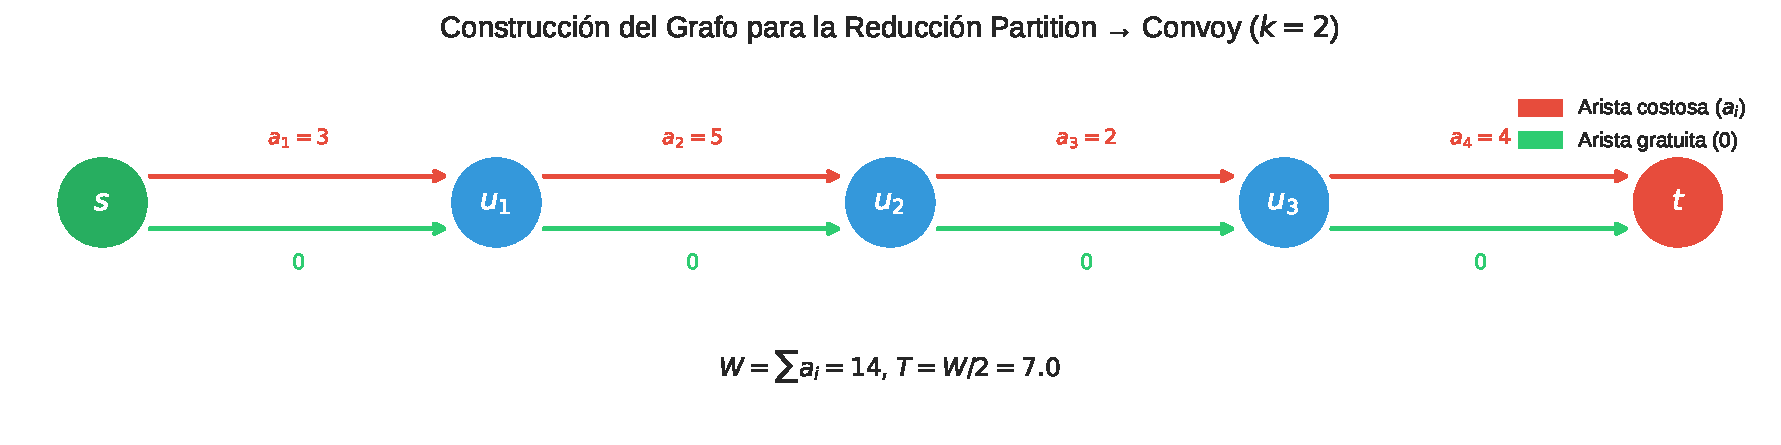
\includegraphics[width=0.95\textwidth]{reduccion_grafo.pdf}
\caption{Construcción del grafo para la reducción Partition $\to$ Convoy. Cada etapa tiene dos aristas paralelas: una con peso $a_i$ (roja) y otra con peso 0 (verde).}
\label{fig:reduccion}
\end{figure}

\subsection{Extensión a $k>2$ vehículos}

\textbf{Nota importante:} La demostración anterior para $k=2$ ya es suficiente para clasificar el problema general como NP-completo (si un caso particular es difícil, el problema general lo es). Sin embargo, para demostrar que el problema sigue siendo difícil para cualquier número fijo de vehículos $k \ge 3$, utilizamos el problema \textsc{$k$-Partition}.

\begin{lemma}[Partition $\propto$ $k$-Partition]
El problema \textsc{Partition} (dividir en 2 conjuntos) se reduce polinomialmente a \textsc{$k$-Partition} (dividir en $k$ conjuntos de igual suma) para cualquier $k > 2$ fijo.
\end{lemma}
\begin{proof}
Sea $A=\{a_1,\dots,a_n\}$ una instancia de \textsc{Partition} con suma total $W$. Queremos saber si existe subconjunto que sume $W/2$.
Construimos una instancia para \textsc{$k$-Partition} añadiendo $k-2$ elementos nuevos ``pesados'', cada uno con valor $W/2$:
\[ A' = A \cup \{ \underbrace{W/2, W/2, \dots, W/2}_{k-2 \text{ elementos}} \} \]
La nueva suma total es $W' = W + (k-2)(W/2) = k(W/2)$. Por lo tanto, el objetivo para cada una de las $k$ partes es $W/2$.
Cualquier solución válida para \textsc{$k$-Partition} debe colocar cada elemento pesado de valor $W/2$ en un subconjunto propio (ya que la suma objetivo es exactamente $W/2$ y los elementos de $A$ son positivos, no caben acompañantes). Así, $k-2$ subconjuntos quedan ocupados por los elementos nuevos. Los elementos originales $A$ deben repartirse obligatoriamente en los 2 subconjuntos restantes, cada uno sumando $W/2$. Esto equivale exactamente a resolver \textsc{Partition} para $A$.
\end{proof}

Gráficamente, hemos ``reservado'' $k-2$ vehículos con cargas triviales y obligamos a resolver el problema difícil con los 2 vehículos restantes.

\paragraph{Construcción del grafo para $k$ vehículos.} Dado un multiconjunto $A=\{a_1,\dots,a_n\}$ con suma $W$, construimos:
\begin{enumerate}
  \item Creamos $n+1$ nodos en secuencia: $u_0=s, u_1, u_2, \dots, u_n=t$.
  \item Para cada etapa $i$ (de $u_{i-1}$ a $u_i$), añadimos exactamente $k$ aristas paralelas:
  \begin{itemize}
    \item Una arista ``costosa'' con peso $w=a_i$.
    \item $k-1$ aristas ``gratuitas'' con peso $w=0$.
  \end{itemize}
  \item El umbral de decisión es $T = W/k$ (asumiendo $k$ divide a $W$; si no, la respuesta es trivialmente NO para partición perfecta).
\end{enumerate}

En cada etapa, los $k$ caminos deben usar aristas distintas (por la condición de disjunción). Como hay exactamente $k$ aristas por etapa, cada camino toma exactamente una. Esto significa:
\begin{itemize}
  \item Exactamente un vehículo ``carga'' el tiempo $a_i$ en la etapa $i$.
  \item Los otros $k-1$ vehículos pasan con coste $0$ en esa etapa.
\end{itemize}

Al final, si $T_j$ es el tiempo total del vehículo $j$, entonces $\sum_{j=1}^k T_j = W$ (cada $a_i$ es cargado por exactamente un vehículo). El problema de minimizar $\max_j T_j$ sujeto a $\sum_j T_j = W$ es equivalente a particionar $\{a_1,\dots,a_n\}$ en $k$ subconjuntos de suma lo más igual posible.

\begin{theorem}
Para cualquier $k\ge 2$ fijo, el problema El Convoy es NP-completo.
\end{theorem}
\begin{proof}
Ya mostramos que está en NP. La reducción desde \textsc{$k$-Way Partition} (NP-completo para $k\ge 2$) sigue la construcción anterior: la instancia de El Convoy tiene solución con $\max T_j \le W/k$ si y sólo si existe una partición perfecta de $A$ en $k$ partes de suma $W/k$.
\end{proof}

\section{Cadena de reducciones: 3-SAT $\to$ Subset Sum $\to$ Partition}
\subsection{\textsc{3-SAT} a \textsc{Subset Sum}}

\begin{definition}[\textsc{3-SAT}]
Entrada: Una fórmula booleana $\phi$ en forma normal conjuntiva (CNF) donde cada cláusula tiene exactamente 3 literales. Pregunta: ¿Existe una asignación de verdad que satisfaga todas las cláusulas?
\end{definition}

\paragraph{Idea intuitiva.} Codificamos cada variable y cada cláusula como ``dígitos'' separados en una representación numérica. Creamos números que representan asignar VERDADERO o FALSO a cada variable, y números auxiliares para ``completar'' las cláusulas. La suma objetivo se alcanza si y sólo si la fórmula es satisfacible.

\paragraph{Construcción formal.} Sea $\phi$ una fórmula 3-SAT con $n$ variables $x_1,\dots,x_n$ y $m$ cláusulas $C_1,\dots,C_m$. Construimos una instancia de \textsc{Subset Sum} así:

\begin{enumerate}
  \item \textbf{Base numérica:} Trabajamos en base $B=10$ (o cualquier $B>3$ para evitar acarreos entre dígitos). Cada número tendrá $n+m$ dígitos: los primeros $n$ corresponden a variables, los últimos $m$ a cláusulas.
  
  \item \textbf{Números para variables:} Para cada variable $x_i$, creamos dos números:
  \begin{itemize}
    \item $v_i$ (representa $x_i = \text{VERDADERO}$): tiene un 1 en la posición $i$ (dígito de variable), y un 1 en la posición $n+j$ por cada cláusula $C_j$ donde $x_i$ aparece \emph{positivo}.
    \item $f_i$ (representa $x_i = \text{FALSO}$): tiene un 1 en la posición $i$, y un 1 en la posición $n+j$ por cada cláusula $C_j$ donde $\neg x_i$ aparece.
  \end{itemize}
  
  \item \textbf{Números auxiliares para cláusulas:} Para cada cláusula $C_j$, creamos dos números auxiliares:
  \begin{itemize}
    \item $s_j^1$: tiene un 1 solo en la posición $n+j$.
    \item $s_j^2$: tiene un 1 solo en la posición $n+j$.
  \end{itemize}
  Estos permiten ``ajustar'' la contribución a cada cláusula.
  
  \item \textbf{Suma objetivo $t$:} Construimos $t$ con:
  \begin{itemize}
    \item Un 1 en cada posición de variable (posiciones $1,\dots,n$): esto fuerza elegir exactamente uno de $\{v_i, f_i\}$ por variable.
    \item Un 3 en cada posición de cláusula (posiciones $n+1,\dots,n+m$): esto fuerza que cada cláusula reciba contribución 3 (al menos 1 de literales + auxiliares).
  \end{itemize}
\end{enumerate}

\paragraph{Ejemplo.} Consideremos $\phi = (x_1 \lor \neg x_2 \lor x_3) \land (\neg x_1 \lor x_2 \lor \neg x_3)$.

Tenemos $n=3$ variables y $m=2$ cláusulas. Los números (en base 10, 5 dígitos: 3 de variables + 2 de cláusulas):

\begin{center}
\begin{tabular}{|c|c|c|}
\hline
Número & Representación & Valor \\
\hline
$v_1$ ($x_1=T$) & $1\ 0\ 0\ |\ 1\ 0$ & 10010 \\
$f_1$ ($x_1=F$) & $1\ 0\ 0\ |\ 0\ 1$ & 10001 \\
$v_2$ ($x_2=T$) & $0\ 1\ 0\ |\ 0\ 1$ & 01001 \\
$f_2$ ($x_2=F$) & $0\ 1\ 0\ |\ 1\ 0$ & 01010 \\
$v_3$ ($x_3=T$) & $0\ 0\ 1\ |\ 1\ 0$ & 00110 \\
$f_3$ ($x_3=F$) & $0\ 0\ 1\ |\ 0\ 1$ & 00101 \\
$s_1^1, s_1^2$ & $0\ 0\ 0\ |\ 1\ 0$ & 00010 \\
$s_2^1, s_2^2$ & $0\ 0\ 0\ |\ 0\ 1$ & 00001 \\
\hline
$t$ (objetivo) & $1\ 1\ 1\ |\ 3\ 3$ & 11133 \\
\hline
\end{tabular}
\end{center}

\paragraph{Corrección de la reducción.}
\begin{itemize}
  \item $(\Rightarrow)$ Si $\phi$ es satisfacible con asignación $\alpha$: Para cada $x_i$, elegimos $v_i$ si $\alpha(x_i)=T$, o $f_i$ si $\alpha(x_i)=F$. Esto da exactamente 1 en cada posición de variable. Para cada cláusula $C_j$, al menos un literal es verdadero, así que recibimos contribución $\ge 1$ de los $v_i/f_i$ elegidos. Usamos auxiliares $s_j^1, s_j^2$ para completar hasta 3.
  
  \item $(\Leftarrow)$ Si existe subconjunto que suma $t$: Las posiciones de variables tienen valor 1 en $t$, y solo $v_i$ y $f_i$ contribuyen a la posición $i$, cada uno con 1. Por lo tanto, elegimos exactamente uno de $\{v_i, f_i\}$ por variable (esto define una asignación $\alpha$). Las posiciones de cláusula tienen valor 3 en $t$, y los auxiliares contribuyen a lo sumo 2 por cláusula. Por lo tanto, al menos 1 debe venir de algún $v_i$ o $f_i$, lo que significa que al menos un literal de cada cláusula es verdadero bajo $\alpha$.
\end{itemize}

\begin{theorem}
\textsc{Subset Sum} es NP-completo.
\end{theorem}
\begin{proof}
Está en NP (verificar suma es polinomial). La reducción desde \textsc{3-SAT} descrita es polinomial: creamos $2n + 2m$ números de $O(n+m)$ dígitos cada uno.
\end{proof}

\subsection{\textsc{Subset Sum} a \textsc{Partition}}
\begin{definition}[\textsc{Subset Sum}]
Entrada: multiconjunto de enteros positivos $S=\{s_1,\dots,s_m\}$ y objetivo $t\in\mathbb{N}$. Pregunta: ¿existe $S'\subseteq S$ tal que $\sum_{x\in S'} x = t$?
\end{definition}

\begin{lemma}[Reducción de Karp]
Dada una instancia $(S,t)$ de \textsc{Subset Sum}, puede construirse en tiempo polinomial una instancia $S^*$ de \textsc{Partition} tal que $S$ admite un subconjunto que suma $t$ si y sólo si $S^*$ es particionable en dos subconjuntos de igual suma.
\end{lemma}
\begin{proof}
Sea $U=\sum_{x\in S} x$. Construimos $S^* = S\cup\{x\}$, donde $x=2t-U$. Si $x\le 0$, aplicamos el truco estándar de sumar una constante $C$ suficientemente grande a todos los elementos y al objetivo para mantener positividad: considere $S' = \{s_i+C\}_{i=1}^m$ y $t' = t + kC$ con $k$ el cardinal del subconjunto; existen formulaciones alternativas que evitan este detalle usando dos elementos $x_1, x_2$ que equilibran la suma.

Suponiendo $x>0$ (la construcción puede garantizarlo), notemos que la suma total en $S^*$ es $U+x=U+2t-U=2t$. Entonces, una partición en dos subconjuntos de igual suma requiere que cada lado sume exactamente $t$. Si existe $S'\subseteq S$ con suma $t$, entonces $S'$ y el complemento $S\setminus S'$ junto con $x$ forman una partición: $\sum S' = t$ y $\sum(S\setminus S') + x = U - t + (2t - U) = t$. Recíprocamente, si existe una partición de $S^*$ en suma $t$ por lado, uno de los lados no puede contener $x$ y elementos adicionales que excedan $t$, por lo que necesariamente selecciona un subconjunto de $S$ que suma $t$. Detalles técnicos para el caso $x\le 0$ se resuelven con las versiones que agregan dos elementos $x_1=t$ y $x_2=U-t$ o mediante codificaciones equivalentes bien conocidas; ver \cite{gareyjohnson}.
\end{proof}

\begin{corollary}
\textsc{Partition} es NP-completo.
\end{corollary}
\begin{proof}
\textsc{Partition} está en NP y recibe reducciones en tiempo polinomial desde \textsc{Subset Sum}, que a su vez recibe reducción desde \textsc{3-SAT}. Por transitividad de las reducciones de Karp, \textsc{Partition} es NP-completo.
\end{proof}

\section{Consecuencias algorítmicas}
Dado que El Convoy es NP-duro, los algoritmos exactos serán exponenciales en el peor caso. Discutimos enfoques prácticos:
\begin{itemize}
  \item \textbf{Fuerza bruta (pequeños $n$):} Enumerar combinaciones de caminos disjuntos y minimizar el máximo.
  \item \textbf{Greedy secuencial:} Encontrar iterativamente el camino más corto disponible (Dijkstra), eliminar sus aristas, repetir $k$ veces.
  \item \textbf{Heurístico aleatorizado:} Variar pesos con pequeñas perturbaciones y elegir múltiples ejecuciones greedy para escapar de óptimos locales.
\end{itemize}

\section{Experimentación}

Para evaluar el desempeño práctico de los algoritmos propuestos, realizamos una serie de experimentos comparando tres enfoques: \textbf{Fuerza Bruta} (exacto, solo para $k=2$), \textbf{Greedy Secuencial} y \textbf{Greedy Aleatorizado}.

\subsection{Metodología}
\begin{itemize}
  \item \textbf{Tipos de grafos:} 
    \begin{enumerate}
      \item \emph{Grafos tipo reducción:} Estructura en etapas con $k$ aristas paralelas por etapa (1 costosa, $k-1$ gratuitas). Representa el peor caso teórico.
      \item \emph{Grafos tipo ciudad (grid):} Malla rectangular que simula calles urbanas con pesos aleatorios.
    \end{enumerate}
  \item \textbf{Métricas:} Tiempo de ejecución (ms) y calidad de solución (gap porcentual respecto al óptimo).
  \item \textbf{Configuración:} Pesos aleatorios en $[1, 100]$, semilla fija para reproducibilidad.
\end{itemize}

\subsection{Resultados de Escalabilidad}

La Tabla \ref{tab:escalabilidad} muestra cómo escala el tiempo de ejecución con el número de etapas $n$ para $k=2$ vehículos.

\begin{table}[h]
\centering
\begin{tabular}{|c|c|c|c|}
\hline
\textbf{Etapas ($n$)} & \textbf{Greedy (ms)} & \textbf{Aleatorizado (ms)} & \textbf{Fuerza Bruta (ms)} \\
\hline
5  & 0.02  & 1.1   & 0.6 \\
8  & 0.05  & 2.4   & 52 \\
10 & 0.06  & 2.5   & 735 \\
12 & 0.05  & 2.3   & 12,835 \\
15 & 0.05  & 2.8   & N/A \\
20 & 0.05  & 3.5   & N/A \\
30 & 0.13  & 8.3   & N/A \\
\hline
\end{tabular}
\caption{Tiempos de ejecución por algoritmo. N/A indica tiempo prohibitivo ($>$ 1 min).}
\label{tab:escalabilidad}
\end{table}

La Figura \ref{fig:escalabilidad} visualiza el crecimiento exponencial de la fuerza bruta comparado con el crecimiento lineal de los heurísticos.

\begin{figure}[H]
\centering
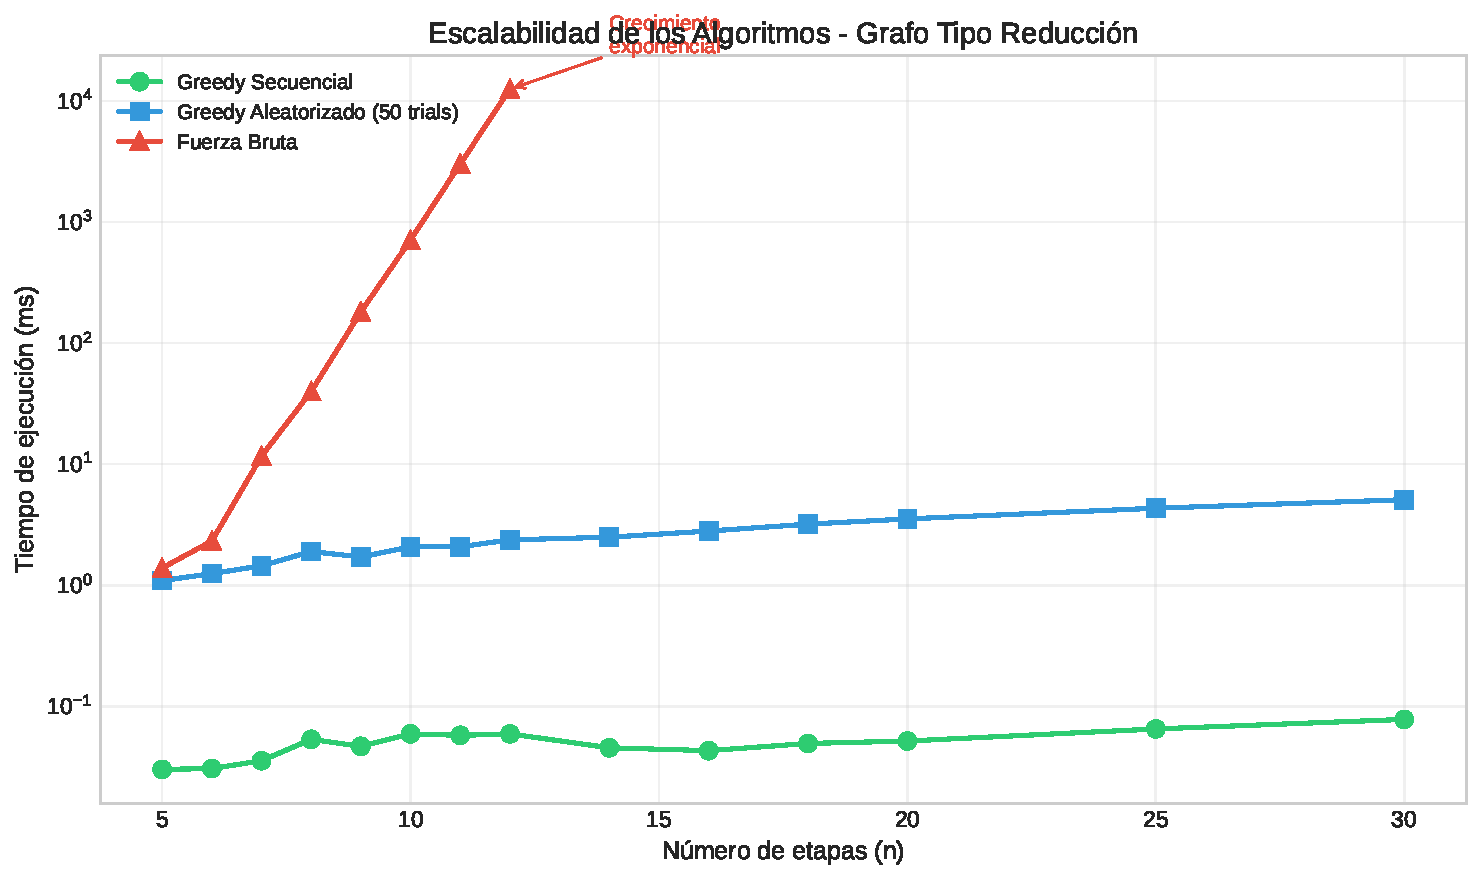
\includegraphics[width=0.85\textwidth]{escalabilidad.pdf}
\caption{Escalabilidad temporal de los algoritmos (escala logarítmica). La fuerza bruta exhibe crecimiento exponencial.}
\label{fig:escalabilidad}
\end{figure}

\textbf{Observaciones:}
\begin{itemize}
  \item \textbf{Fuerza Bruta} exhibe crecimiento exponencial: de 0.6 ms ($n=5$) a casi 13 segundos ($n=12$). Para $n \ge 15$ es impracticable.
  \item \textbf{Greedy Secuencial} es extremadamente rápido ($< 0.2$ ms incluso para $n=30$), con complejidad $O(k \cdot (|V|+|E|) \log |V|)$.
  \item \textbf{Greedy Aleatorizado} escala linealmente con el número de trials (50 en estos experimentos).
\end{itemize}

\subsection{Calidad de las Soluciones}

La Tabla \ref{tab:calidad} muestra el gap porcentual respecto al óptimo (Fuerza Bruta) en grafos tipo reducción.

\begin{table}[h]
\centering
\begin{tabular}{|c|c|c|c|}
\hline
\textbf{Algoritmo} & \textbf{Gap Promedio} & \textbf{Gap Máximo} & \textbf{Gap Mínimo} \\
\hline
Greedy Secuencial    & +98.96\% & +100.00\% & +95.07\% \\
Greedy Aleatorizado  & +98.96\% & +100.00\% & +95.07\% \\
\hline
\end{tabular}
\caption{Gap respecto al óptimo en grafos tipo reducción ($n=8$, $k=2$, 20 instancias).}
\label{tab:calidad}
\end{table}

\textbf{Análisis:} En los grafos tipo reducción, los algoritmos greedy tienen un gap cercano al 100\%. Esto es esperado: la estructura del grafo (aristas paralelas) genera un ``peor caso'' donde el greedy siempre elige la arista de costo 0, dejando todas las aristas costosas para el segundo camino. Este es precisamente el comportamiento que demuestra la NP-dureza del problema.

La Figura \ref{fig:calidad} muestra el gap por instancia, y la Figura \ref{fig:comparacion} compara el rendimiento en diferentes tipos de grafos.

\begin{figure}[H]
\centering
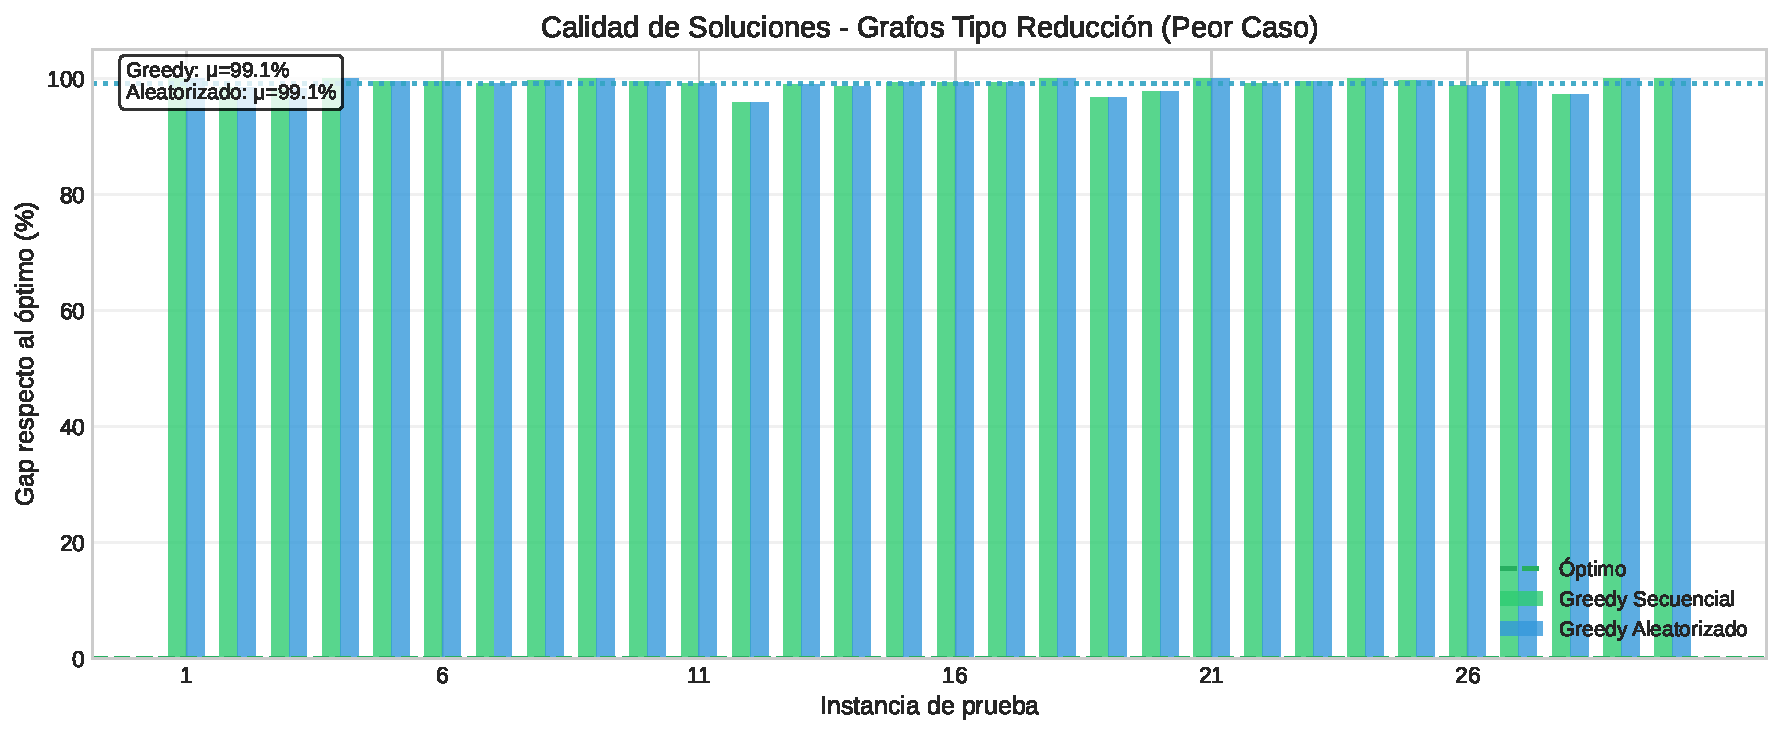
\includegraphics[width=0.9\textwidth]{calidad_soluciones.pdf}
\caption{Gap respecto al óptimo por instancia en grafos tipo reducción. Los heurísticos son consistentemente subóptimos en este peor caso.}
\label{fig:calidad}
\end{figure}

\begin{figure}[H]
\centering
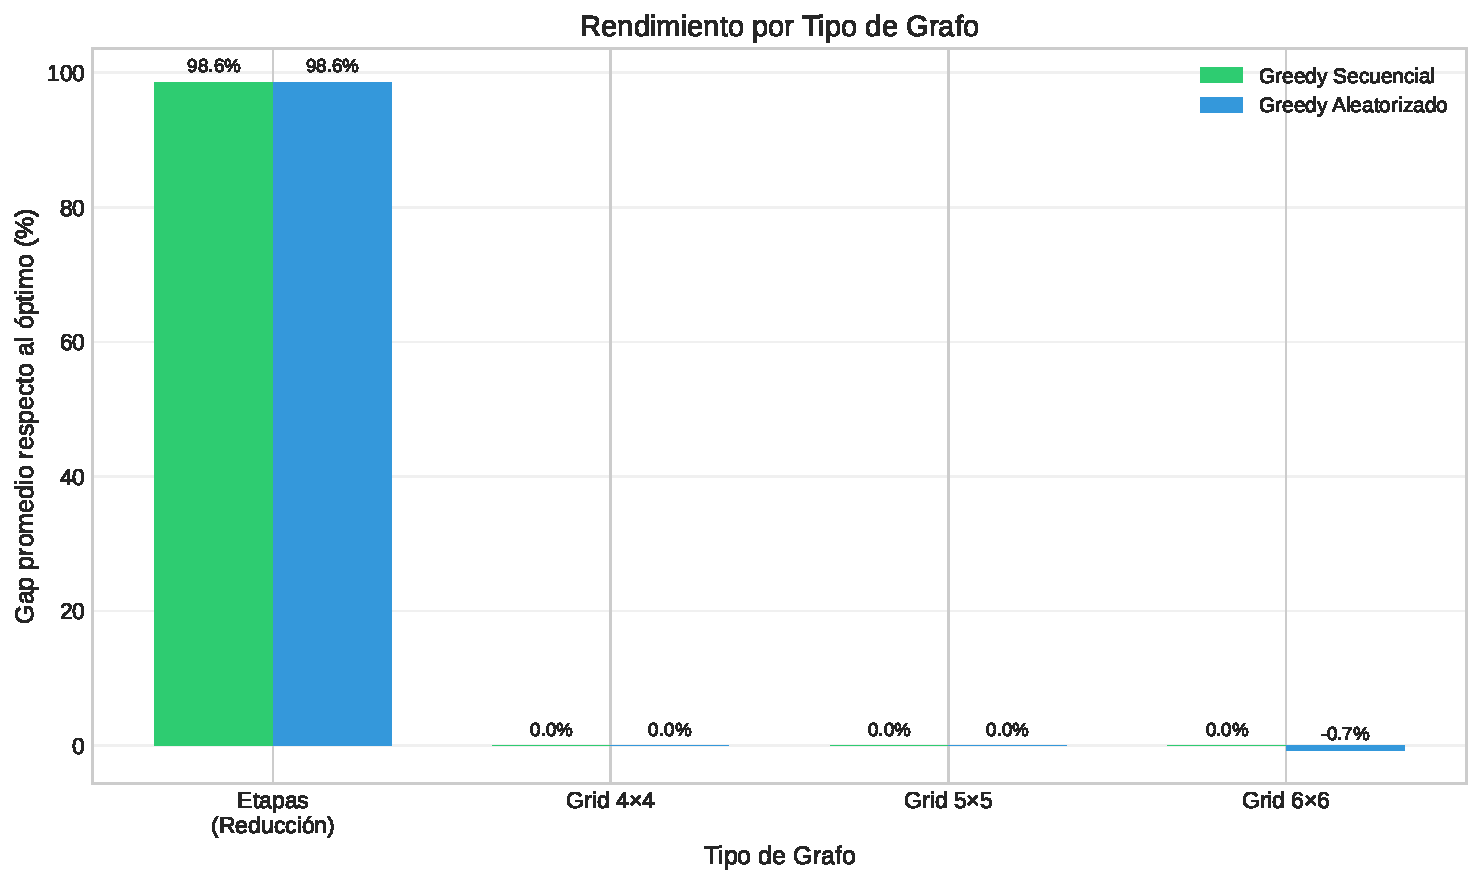
\includegraphics[width=0.85\textwidth]{comparacion_grafos.pdf}
\caption{Comparación del gap promedio por tipo de grafo. Los grafos tipo reducción representan el peor caso; los grids son más favorables.}
\label{fig:comparacion}
\end{figure}

\subsection{Grafos Realistas (Grid)}

En grafos tipo ciudad (malla 4$\times$4), los resultados son más favorables para los heurísticos:

\begin{table}[h]
\centering
\begin{tabular}{|c|c|c|}
\hline
\textbf{Algoritmo} & \textbf{Max Costo} & \textbf{Tiempo (ms)} \\
\hline
Greedy Secuencial    & 119 & 0.07 \\
Greedy Aleatorizado  & 119 & 4.60 \\
Fuerza Bruta         & 119 & 0.35 \\
\hline
\end{tabular}
\caption{Resultados en grafo grid 4$\times$4 con $k=2$.}
\label{tab:grid}
\end{table}

En este caso, los tres algoritmos encuentran la misma solución óptima, lo que sugiere que en grafos con mayor conectividad (más rutas alternativas), los heurísticos pueden ser efectivos.

\subsection{Conclusiones Experimentales}
\begin{enumerate}
  \item \textbf{Fuerza Bruta} es viable solo para instancias muy pequeñas ($n \le 12$).
  \item \textbf{Greedy Secuencial} es el más rápido pero puede dar soluciones muy subóptimas en grafos adversariales.
  \item \textbf{Greedy Aleatorizado} ofrece un balance entre tiempo y calidad, especialmente útil cuando se dispone de tiempo para múltiples iteraciones.
  \item La estructura del grafo influye significativamente: grafos más conectados favorecen a los heurísticos.
\end{enumerate}

\section{Referencias}
\begin{thebibliography}{9}
\bibitem{gareyjohnson} M. R. Garey, D. S. Johnson. \emph{Computers and Intractability: A Guide to the Theory of NP-Completeness}. W. H. Freeman, 1979.
\end{thebibliography}

\end{document}
